\section{Weights distribution}

\subsection{Model}
\begin{frame}  
    \frametitle{Mnist handwritten database}
	\begin{itemize}
		\item Two convolutional layers.
		\item Two max pooling layers.   
		\item Two dense layers.  
		\item One dropout layer.
	\end{itemize}
\end{frame}

\subsection{Initial}
\begin{frame}
    \frametitle{Initial}
    	\begin{figure}
		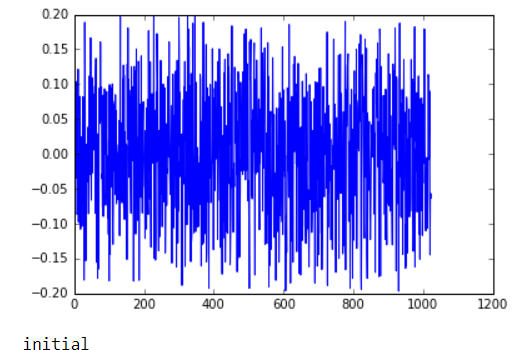
\includegraphics[scale=0.3]{figure/Initial.PNG}
	\end{figure}
\end{frame}

\subsection{Iteration 50}
\begin{frame}
    \frametitle{Weights and gradients}
    \begin{figure}
		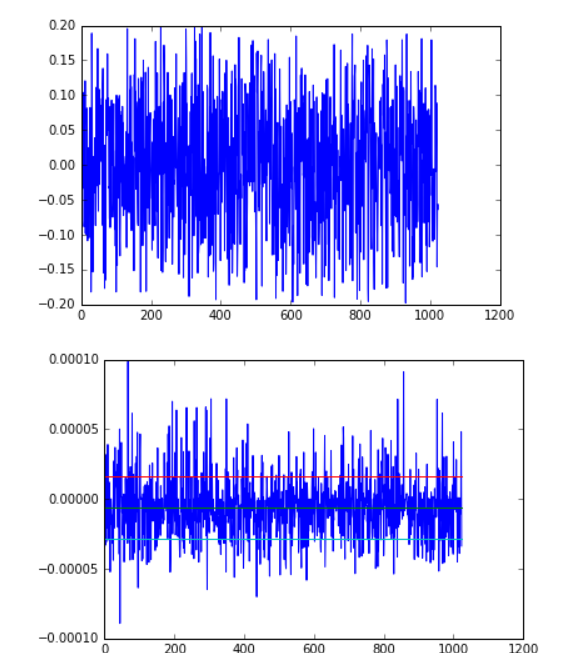
\includegraphics[scale=0.3]{figure/50-1.PNG}
\end{figure}
\end{frame}
\begin{frame}
    \frametitle{Gradients distribution}
    \begin{figure}
		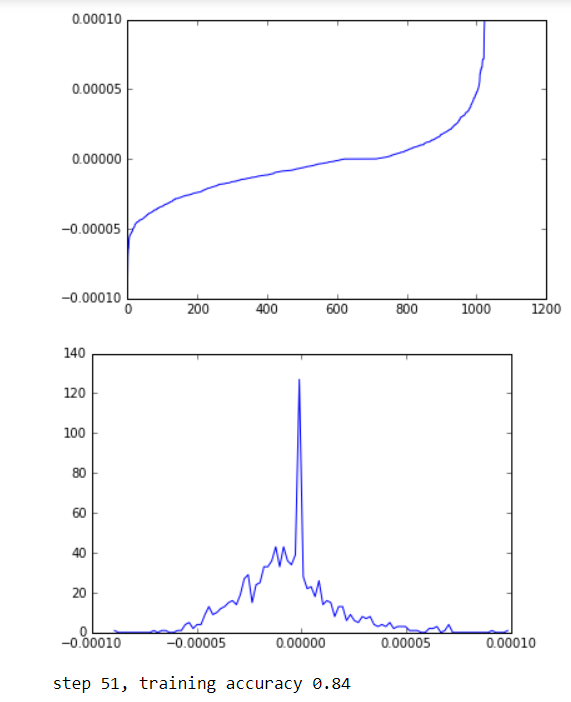
\includegraphics[scale=0.28]{figure/50-2.PNG}
    \end{figure}
\end{frame}

\subsection{Iteration 200}
\begin{frame}
    \frametitle{Weights and gradients}
    \begin{figure}
		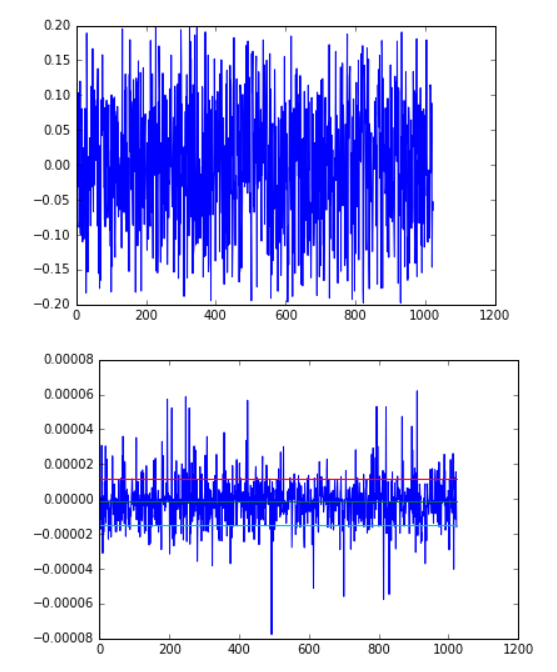
\includegraphics[scale=0.3]{figure/200-1.PNG}
    \end{figure}
\end{frame}
\begin{frame}

    \frametitle{Gradients distribution}
    \begin{figure}
		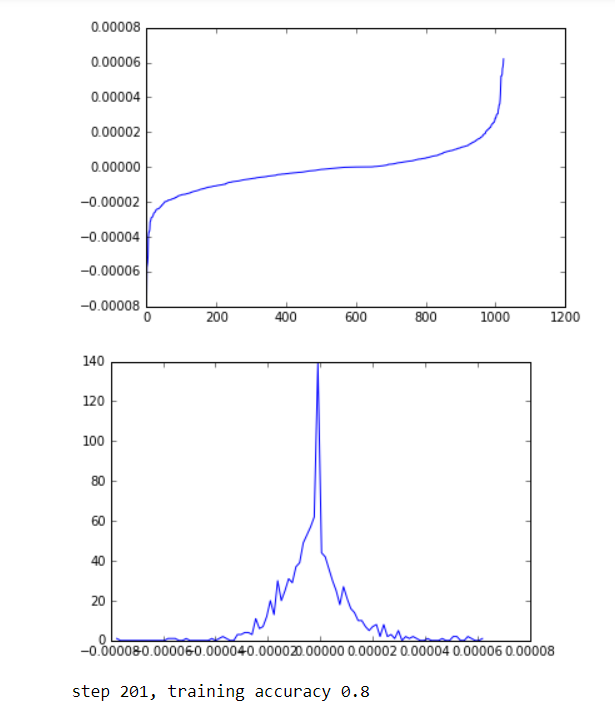
\includegraphics[scale=0.28]{figure/200-2.PNG}
    \end{figure}
\end{frame}
\subsection{Iteration 550}
\begin{frame}
    \frametitle{Weights and gradients}
    \begin{figure}
		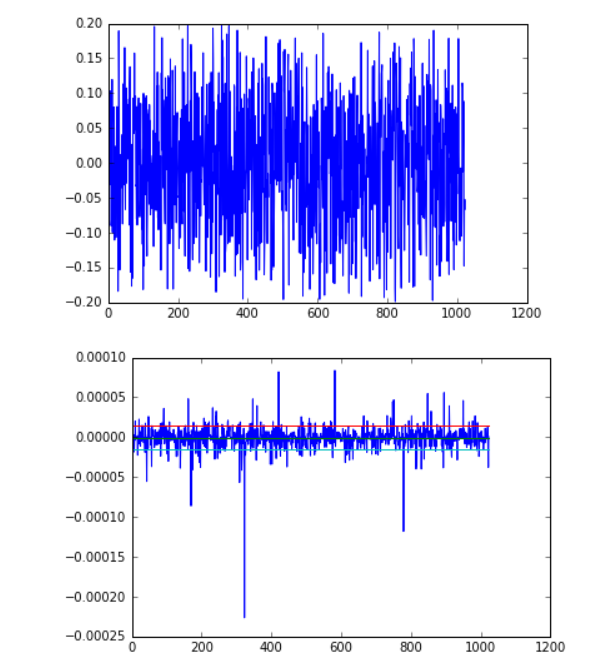
\includegraphics[scale=0.3]{figure/551-1.PNG}
    \end{figure}
\end{frame}
\begin{frame}

    \frametitle{Gradients distribution}
    \begin{figure}
		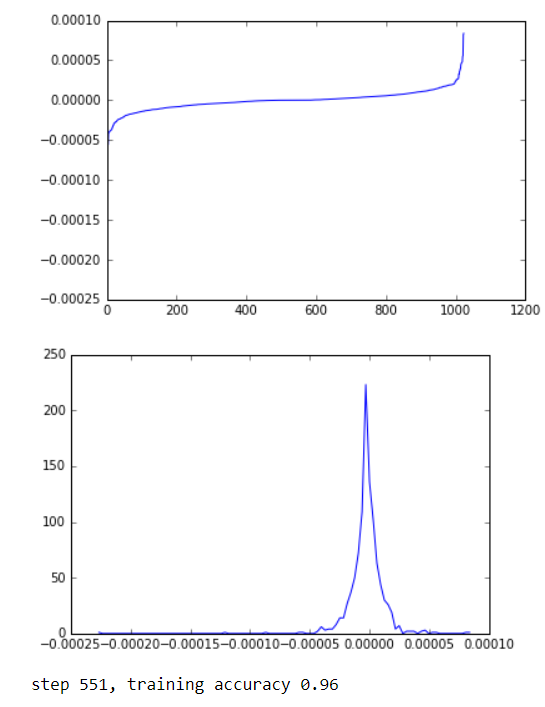
\includegraphics[scale=0.28]{figure/551-2.PNG}
    \end{figure}
\end{frame}
\subsection{Iteration 950}
\begin{frame}
    \frametitle{Weights and gradients}
    \begin{figure}
		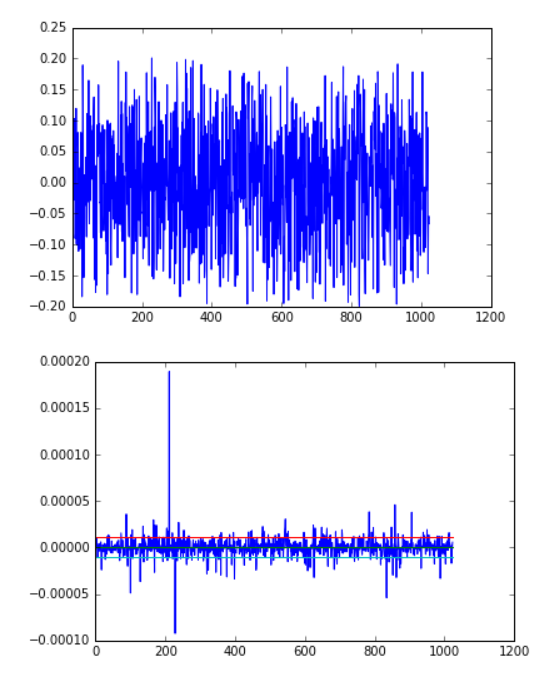
\includegraphics[scale=0.3]{figure/951-1.PNG}
    \end{figure}
\end{frame}
\begin{frame}

    \frametitle{Gradients distribution}
    \begin{figure}
		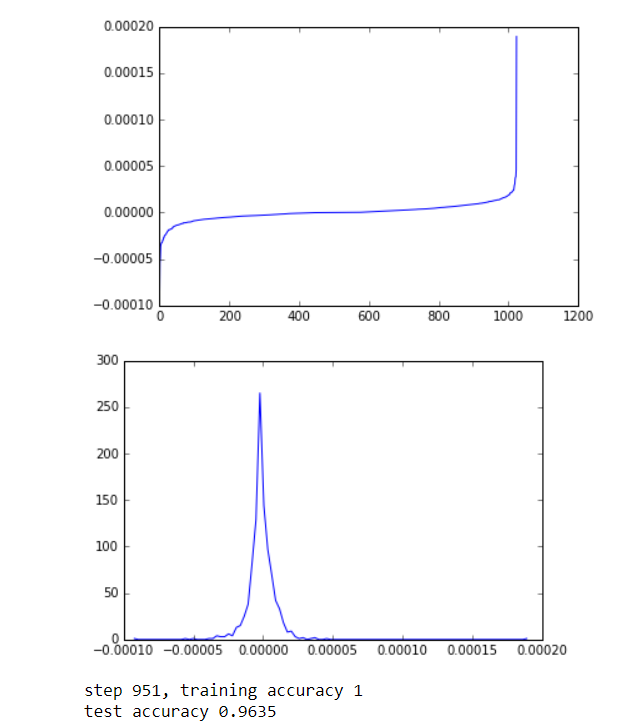
\includegraphics[scale=0.28]{figure/951-2.PNG}
    \end{figure}
\end{frame}

